%\documentclass[10pt,a4paper]{amsart}
\documentclass[onetab, a4paper]{siamart171218}
% review for line numbers
\usepackage[cm, headings]{fullpage}
\usepackage{lineno}
\usepackage{chngcntr}
\usepackage{amsopn}
\usepackage{amsmath}
\usepackage{amssymb}
\usepackage{graphicx}
\usepackage{capt-of}
%\usepackage[table]{xcolor}% http://ctan.org/pkg/xcolor
%\usepackage{tabularx}
%\usepackage{booktabs}
\usepackage{multirow}
\usepackage{makecell}
\usepackage{multicol}
\usepackage{float}
\usepackage{todonotes}
\usepackage{chngcntr}
\usepackage{multicol}
%\usepackage{amsthm}
\usepackage{cleveref}
\usepackage{url}
%\usepackage{mathtools}

\usepackage{tikz}
\usetikzlibrary{calc}
\usetikzlibrary{shapes, snakes, patterns, arrows}

\usepackage{varwidth}
\newsavebox\tmpbox

\usepackage{thm-restate}
%\counterwithin{table}{subsection}
\usepackage{algpseudocode}  % gets
\usepackage[utf8]{inputenc}

\newcommand{\dual}{'}
\newcommand{\reals}{{\mathbb{R}}}
\newcommand{\abs}[1]{\lvert#1\rvert}
\newcommand{\semi}[1]{\lvert#1\rvert}
\newcommand{\norm}[1]{\lVert#1\rVert}
\newcommand{\eps}{\varepsilon}
\newcommand{\set}[1]{\{#1\}}

\newtheorem{thm}{Theorem}[section]
\newtheorem{prop}{Property}[section]
\theoremstyle{remark}
\newtheorem{remark}{Remark}[section]

\newtheorem{example}{Example}[section]

\usepackage{chngcntr}
\counterwithin{table}{section}

\DeclareGraphicsRule{*}{eps}{*}{}

\title{Training Yarotstky networks
  \thanks{Submitted to the editors DATE.
\funding{This work was funded by ...}}
}

% Sets running headers as well as PDF title and authors
\headers{}{}

% Authors: full names plus addresses.
\author{Authors\thanks{
    Simula Research Laboratory, Fornebu, Norway}
}

\usepackage{amsopn}
\DeclareMathOperator{\diag}{diag}


%\author{Karl Erik Holter \and Miroslav Kuchta \and Kent-Andre Mardal}

\begin{document}

\maketitle 
\begin{abstract}
  {
    It seems difficult
}
\end{abstract}

\begin{keywords}
neural networks, stochastic gradient descent
\end{keywords}

% REQUIRED
\begin{AMS}
n.a.
\end{AMS}

\section{Introduction}

Paper \cite{yarotsky2017error} constructs approximation of $x^2$ on a
unit interval in terms of a particular deep neural network, here termed
$\mathcal{Y}_m$, of depth $m$ and using ReLU as activation function.
Utilizing skip connections, each hidden layer has a fixed width of 3
neurons and the affine mapping between \emph{any} two consecutive hidden
layers is given by a matrix
\[
A = \begin{pmatrix}
  2& -4& 2\\
  2& -4& 2\\
  2& -4& 2\\  
  \end{pmatrix}.
\]
It is shown that $\norm{x^2 - \mathcal{Y}_m} \lesssim 2^{-m}$ and the
convergence properties are due to the fact that the network effectively
constructs the approximation as a linear combination of sawtooth functions
$g_m=\underbrace{g\circ g \circ \cdots \circ g}_{m}$ where $g$ is piecewise
linear hat function. The linear combination and composition ideas are mirrored
in the construction of the network: the ouput of each $k$-th hidden layer is both
contracted (to form $g_k$) and propagated forward by $A$ (to contribute
to $g_{k+1}$). The contraction is done by bector $b=(2, -4, 2)$.

The question we address here is whether $\mathcal{Y}_m$ can be obtained by training with
stochastic gradient descent (or other standard optimizers using in the
field of deep learning).

\subsection{Architectures} We shall always seek the Yarotsky network $\mathcal{Y}_m$
among networks with $m$ hidden layers of width 3 such that output of each hidden
layer $i$ is both propagated forward (to layer $j=i+1$) by affine mapping $x\mapsto A_{ij}x+b_{ij}$ where
$A_{ij}\in\reals^{3, 3}$, $b_{ij}\in\reals^{3}$ and contracted using
$x\mapsto A_{i}x+b_{i}$ where $A_{i}\in\reals^{3}$, $b_{i}\in\reals$.
Results of contraction are combined in the final layer to form the linear
combination that is the network's output.

To push the network towards $\mathcal{Y}_m$ we shall in the \emph{shared}
architecture, $\mathcal{S}_m$, set $A_{ij}=A$, $b_{ij}=b$, $A_{i}=\hat{A}$ and $b_{i}=\hat{b}$,
i.e. share the weights for contraction and propagation. The degrees of freedom
of the shared constuction are thus $A$, $b$, $\hat{A}$, $\hat{b}$ and the weights
to form the linear combination. In the other case the affine maps can be
different from one layer to another. These networks shall be denoted as
$\mathcal{N}_m$.

\subsection{Training set} We will consider two ways of generating the training
data. In the \emph{random} case we draw the points randonly from unit interval.
In \emph{uniform} case we let $y_i$ by the equispaced points in $(0, 1)$. The
training set is then $\sqrt{y_i}$. In both we include the boundary points in the
training set.

\subsection{Regularization} Given training points $x_i$, $i\in I$, the
objective for the optimizer (Adam \cite{kingma2014adam}) that we used is
\[
E(\mathcal{N}, I) = \overline{\sum_i(x^2_i - \mathcal{N}(x_i))^2} + \lambda \sum_{i}\text{tr}(A^T_{i, i+1} A_{i, i+1}),
\]
where the overline denotes the ansemble mean and $\lambda$ is fixed.

\subsection{Training procedure} To account for the increased number of
weights with $m$ the number of steps of the optimizer as well as the batch
size, i.e $\norm{I}$, depend on $m$. The former grows with logarithm of
$m$ while the later depends linearly on the depth.

\section{Results} Our observations are summarized in Figure \ref{fig:comparison}.
(i) It can be seen that none of the trained networks for $m>2$ comes close to the
error of $\mathcal{Y}_m$. (ii) The shared networks $\mathcal{S}_m$, which
in theory have an architecture closer to $\mathcal{Y}_m$ do not in general yield
smaller error than $\mathcal{N}_m$. (iii) Training with random points in the training
set leads to smaller error then if mapped equispaced points are used. (iv) Comparing
$\lambda=0$ and $\lambda=10^{-6}$ the regulatization does not have a considerable
effect.

\begin{figure}
  \begin{center}
  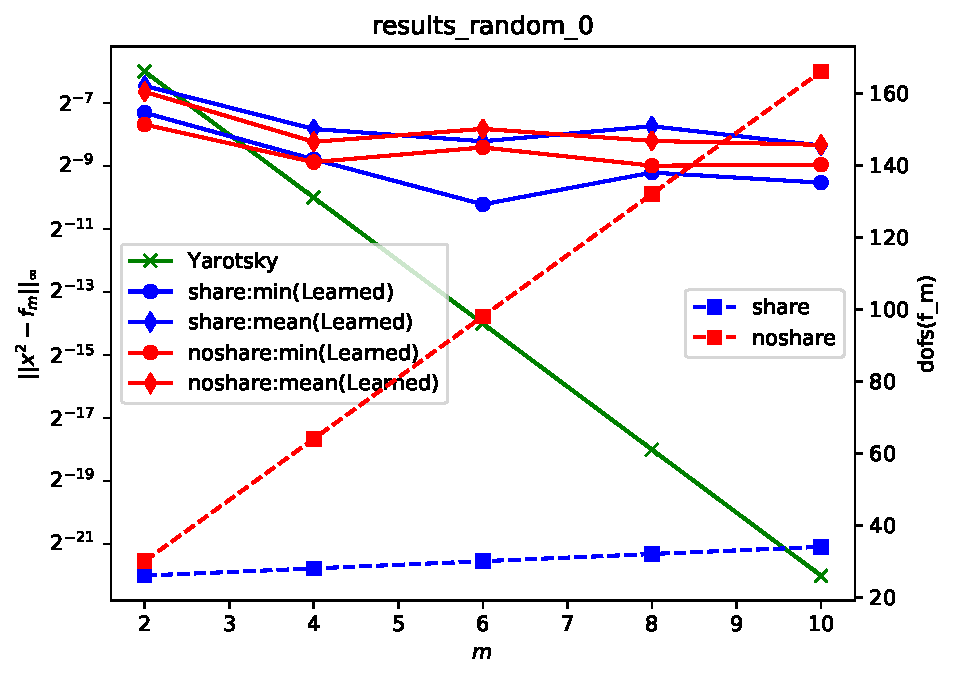
\includegraphics[width=0.45\textwidth]{./img/results_random_0}
  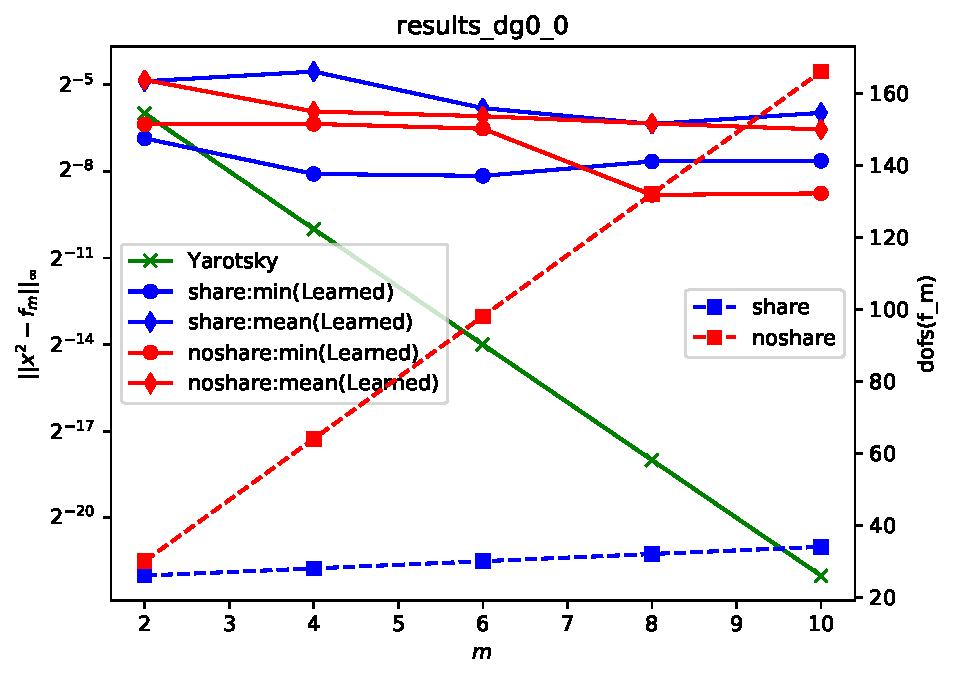
\includegraphics[width=0.45\textwidth]{./img/results_dg0_0}\\
  %
  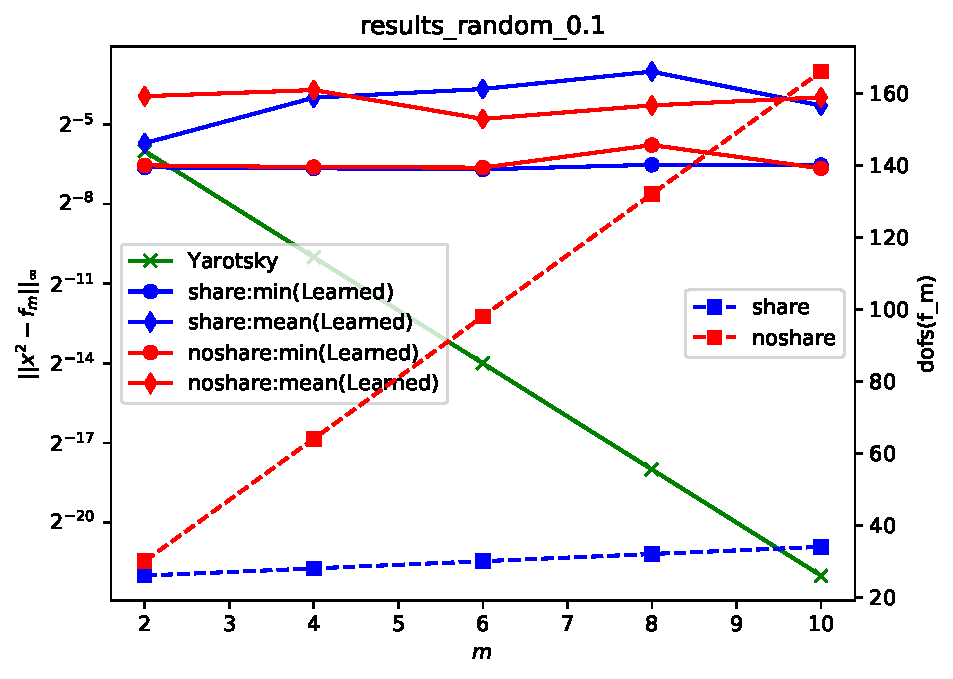
\includegraphics[width=0.45\textwidth]{./img/results_random_01}
  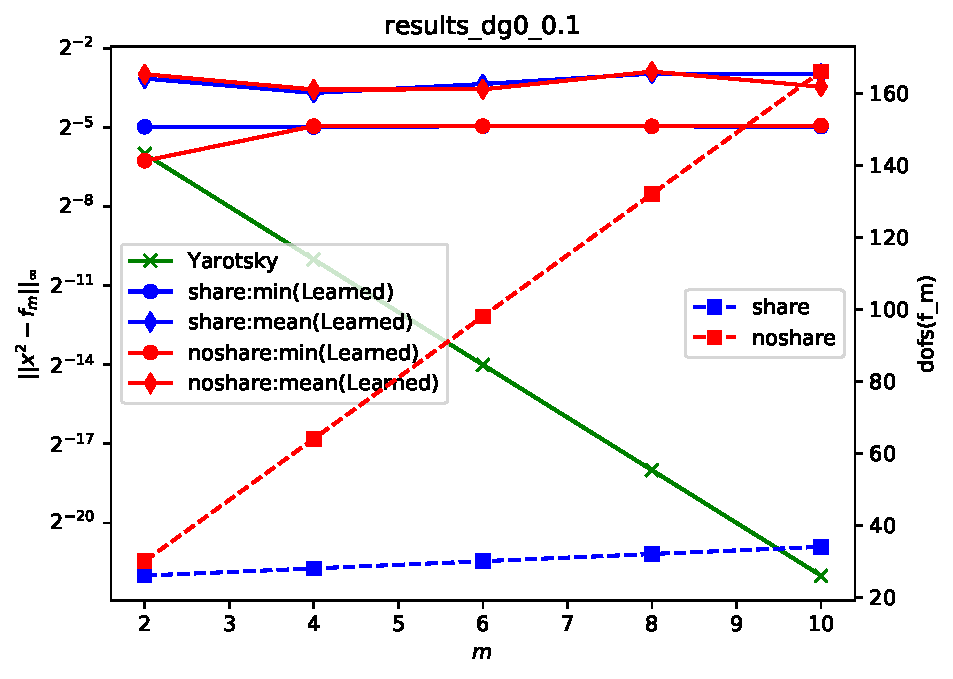
\includegraphics[width=0.45\textwidth]{./img/results_dg0_01}\\
  %
  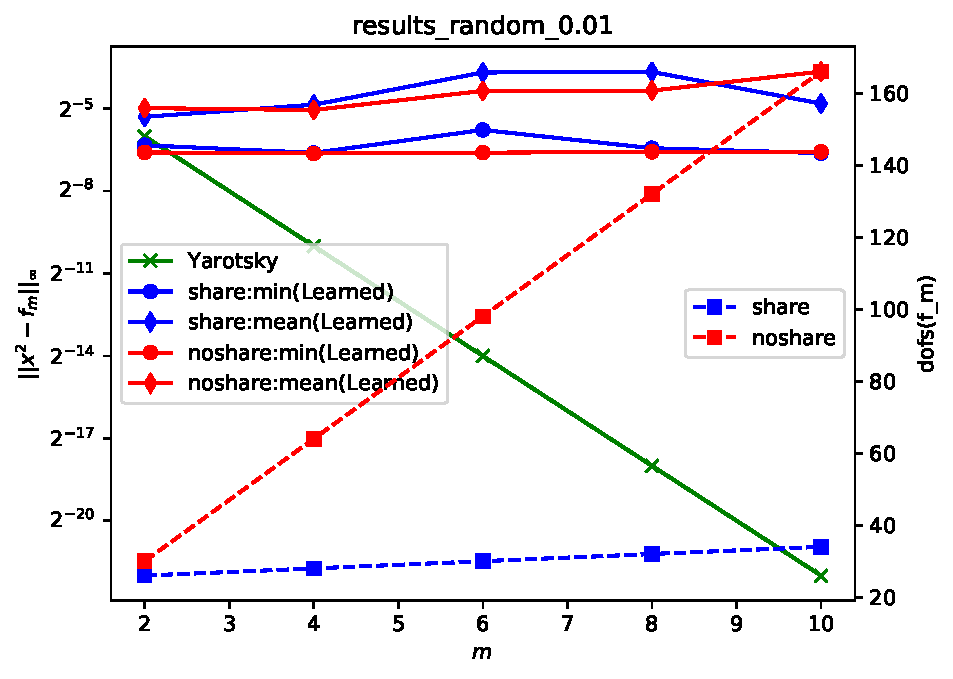
\includegraphics[width=0.45\textwidth]{./img/results_random_001}
  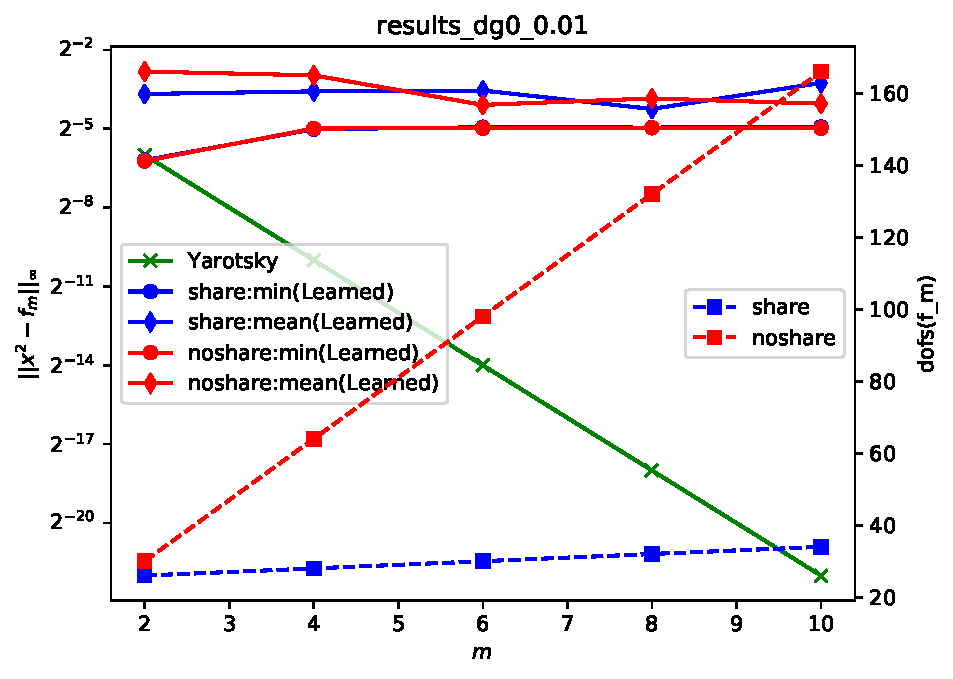
\includegraphics[width=0.45\textwidth]{./img/results_dg0_001}\\
  %
  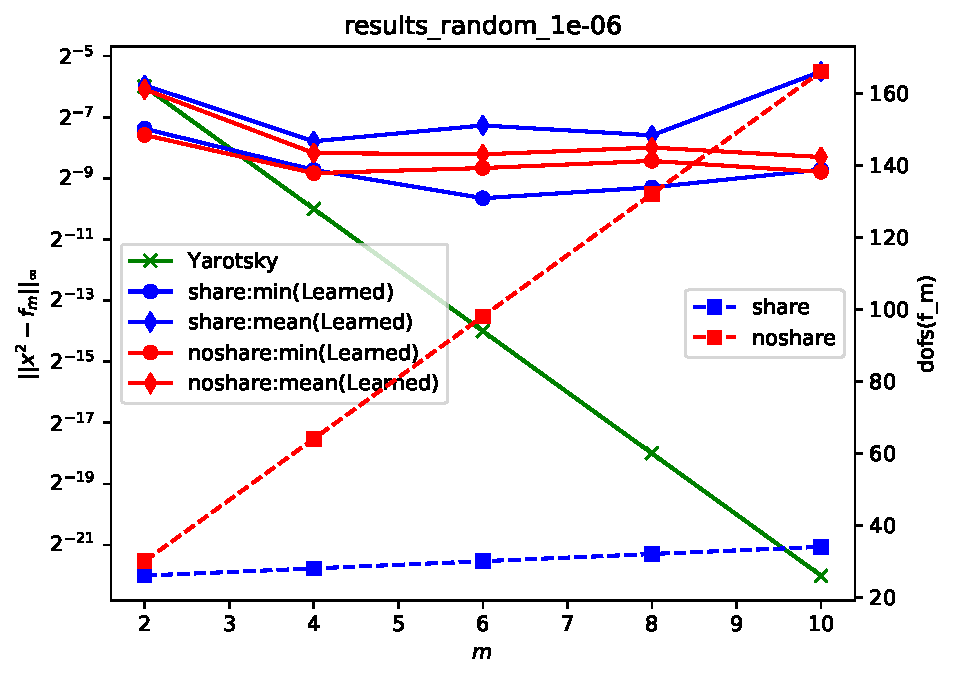
\includegraphics[width=0.45\textwidth]{./img/results_random_1e-06}
  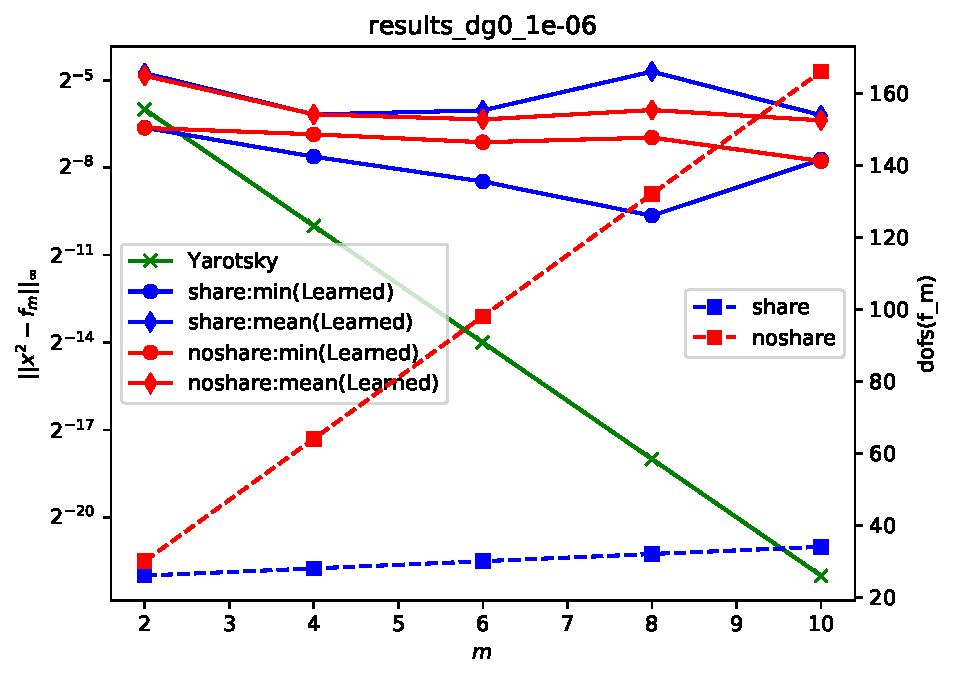
\includegraphics[width=0.45\textwidth]{./img/results_dg0_1e-06}\\
  \end{center}
  \caption{Approximation properties of trained networks. Ten networks
    for each architecture are trained. (Left) Random
    points in the training set. (Right) Equispaced points mapped by $\sqrt{}$.
    Penalty $\lambda$ is different in rows.}
  \label{fig:comparison}
\end{figure}

\newpage
\section{Ideas}
\begin{itemize}
  \item Hierarchy: train $\mathcal{N}_2$. Use its weights init training $\mathcal{N}_3$.
\end{itemize}


\bibliographystyle{siamplain}
\bibliography{yarotsky}

\end{document}
